%!TEX TS-program = xelatex
%!TEX encoding = UTF-8 Unicode
\documentclass[12pt,a4paper]{awesome-cv}
\usepackage{graphicx}
\usepackage{caption}
\DeclareCaptionFont{statement}{\fontsize{9pt}{11pt}\bodyfont\color{black}}
\captionsetup{font=statement,labelfont=bf,skip=5pt,hypcap=false}
\setlength{\textfloatsep}{6pt}

\geometry{left=1.4cm,right=1.4cm,top=0.8cm,bottom=1.8cm,footskip=0.5cm}
\fontdir[fonts/]
\colorlet{awesome}{awesome-blue}
\definecolor{darktext}{HTML}{2B2B2B}
\renewcommand{\acvHeaderSocialSep}{\quad\textbar\quad}
\renewcommand*{\lettertextstyle}{\fontsize{11pt}{14pt}\bodyfont\upshape\color{black}}
\renewcommand*{\lettertitlestyle}[1]{{\fontsize{14pt}{18pt}\bodyfont\bfseries\color{darktext}\underline{#1}}}
\hypersetup{
  pdftitle={Research Statement},
  pdfauthor={Jacob Tutt}
}

\name{Jacob}{Tutt}
\position{AI4Science PhD Researcher\enskip\cdotp\enskip{\href{https://www.kicc.cam.ac.uk}{Kavli Institute for Cosmology}}\enskip\cdotp\enskip Cavendish Laboratory\enskip\cdotp\enskip{\href{https://www.cam.ac.uk/}{University of Cambridge}}}
\address{Battcock Centre, Cavendish Laboratory, JJ Thomson Avenue, Cambridge, CB3 0HE, UK}
\mobile{(+44) 7392 829036}
\email{jlt67@cam.ac.uk}
\homepage{jacobtutt.github.io}
\github{JacobTutt}
\linkedin{jacobltutt}

\recipient{}{\strut}
\letterdate{\today}
\lettertitle{Research Statement}
\letteropening{\strut}

\begin{document}
\makecvheader[R]
\makecvfooter{\today}{Jacob Tutt~~~\textperiodcentered~~~Research Statement}{\thepage}
\par\vspace{1mm}
\noindent\lettertitlestyle{Research Statement}\hfill\letterdatestyle{\today}\par
\vspace{1mm}

\begin{cvletter}
Cosmologists have mapped the bookends of the Universe's history in remarkable detail. At one end, measurements of the Cosmic Microwave Background have enabled precise constraints to be placed on the initial conditions and physical processes governing its prior evolution. At the other, galaxy surveys have revealed the richly structured web of galaxies, filaments and voids that surround us today. Yet the timing and physics connecting these epochs remain poorly constrained, from the formation of the first stars and galaxies to their heating and ionisation of the surrounding gas. 21-cm cosmology offers a uniquely powerful route to reconstructing this history by measuring not the individual sources themselves, but the faint radio signal from the neutral hydrogen surrounding them, tracing both its evolution and its spatial fluctuations.

However, realising this potential poses a notoriously challenging inference problem. The cosmological signal lies buried beneath contaminating emission four to five orders of magnitude brighter, and is observed through a complex instrumental response that strongly mixes contributions, rendering them highly degenerate in the observed data. Given the nuisance contributions cannot be sufficiently constrained a priori, 21-cm signal detection and characterisation are acutely sensitive to model misspecification. Reliable inference therefore demands a unified model of the full observational chain, spanning uncertainties in astrophysical emission, computational electromagnetics and electrical engineering.

End-to-end inference at the required scale and physical fidelity has previously been intractable. My research tackles this problem by combining computational statistics, machine learning and distributed computing. I develop physically motivated, differentiable and hardware-accelerated generative models, alongside scalable Bayesian inference methods for exploring the high-dimensional, multimodal posteriors that arise. More broadly, I am motivated by the challenge of scaling statistical and numerical methods across physics, both algorithmically and computationally, to ever larger datasets, parameter spaces and physical systems.

As part of the Radio Experiment for the Analysis of Cosmic Hydrogen (REACH), I lead the development of its differentiable, hardware-accelerated Bayesian analysis pipeline, built to address a computational bottleneck that had limited the scale and fidelity of the inference needed for a trusted global 21-cm detection.
\par
\begin{figure}[!b]
\centering
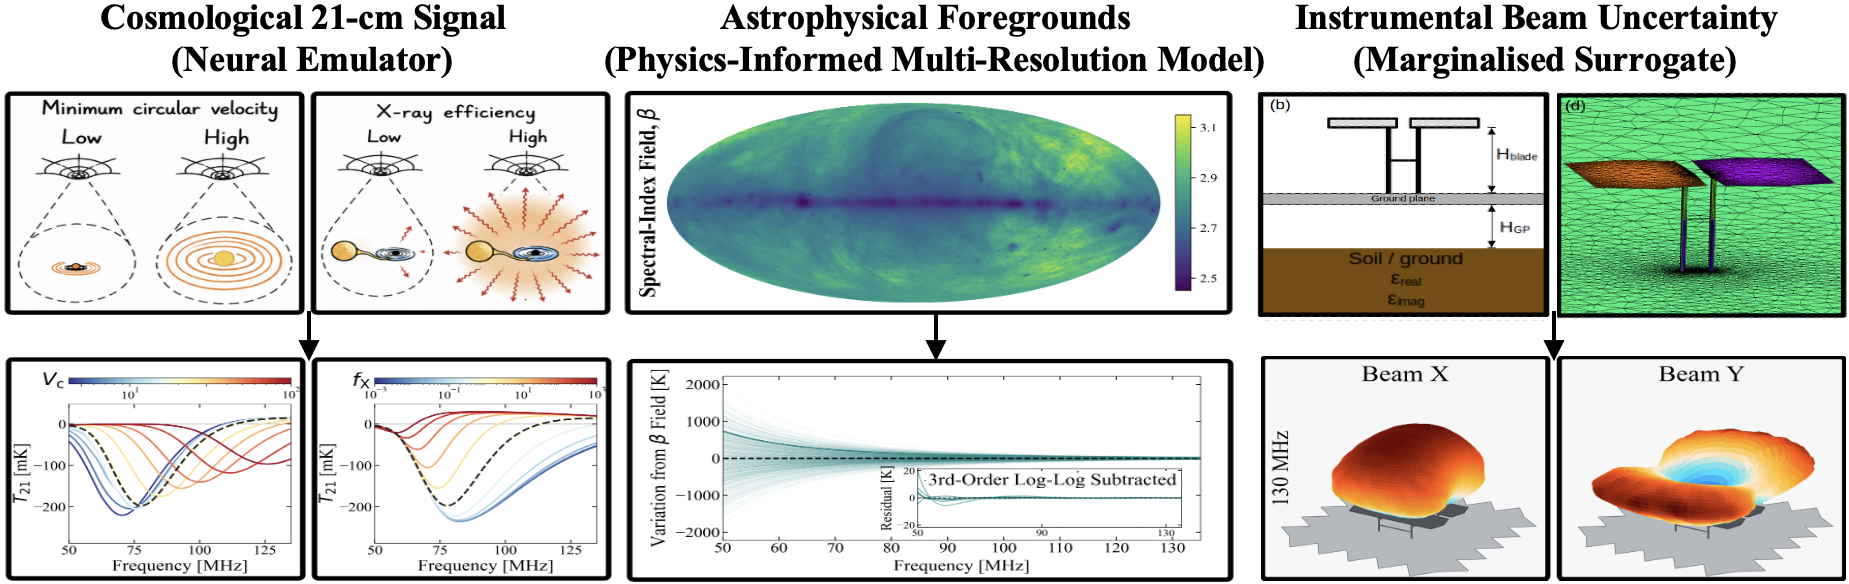
\includegraphics[width=0.9\linewidth,height=43mm]{figures/reach_forward_model.png}\par\vspace{1mm}
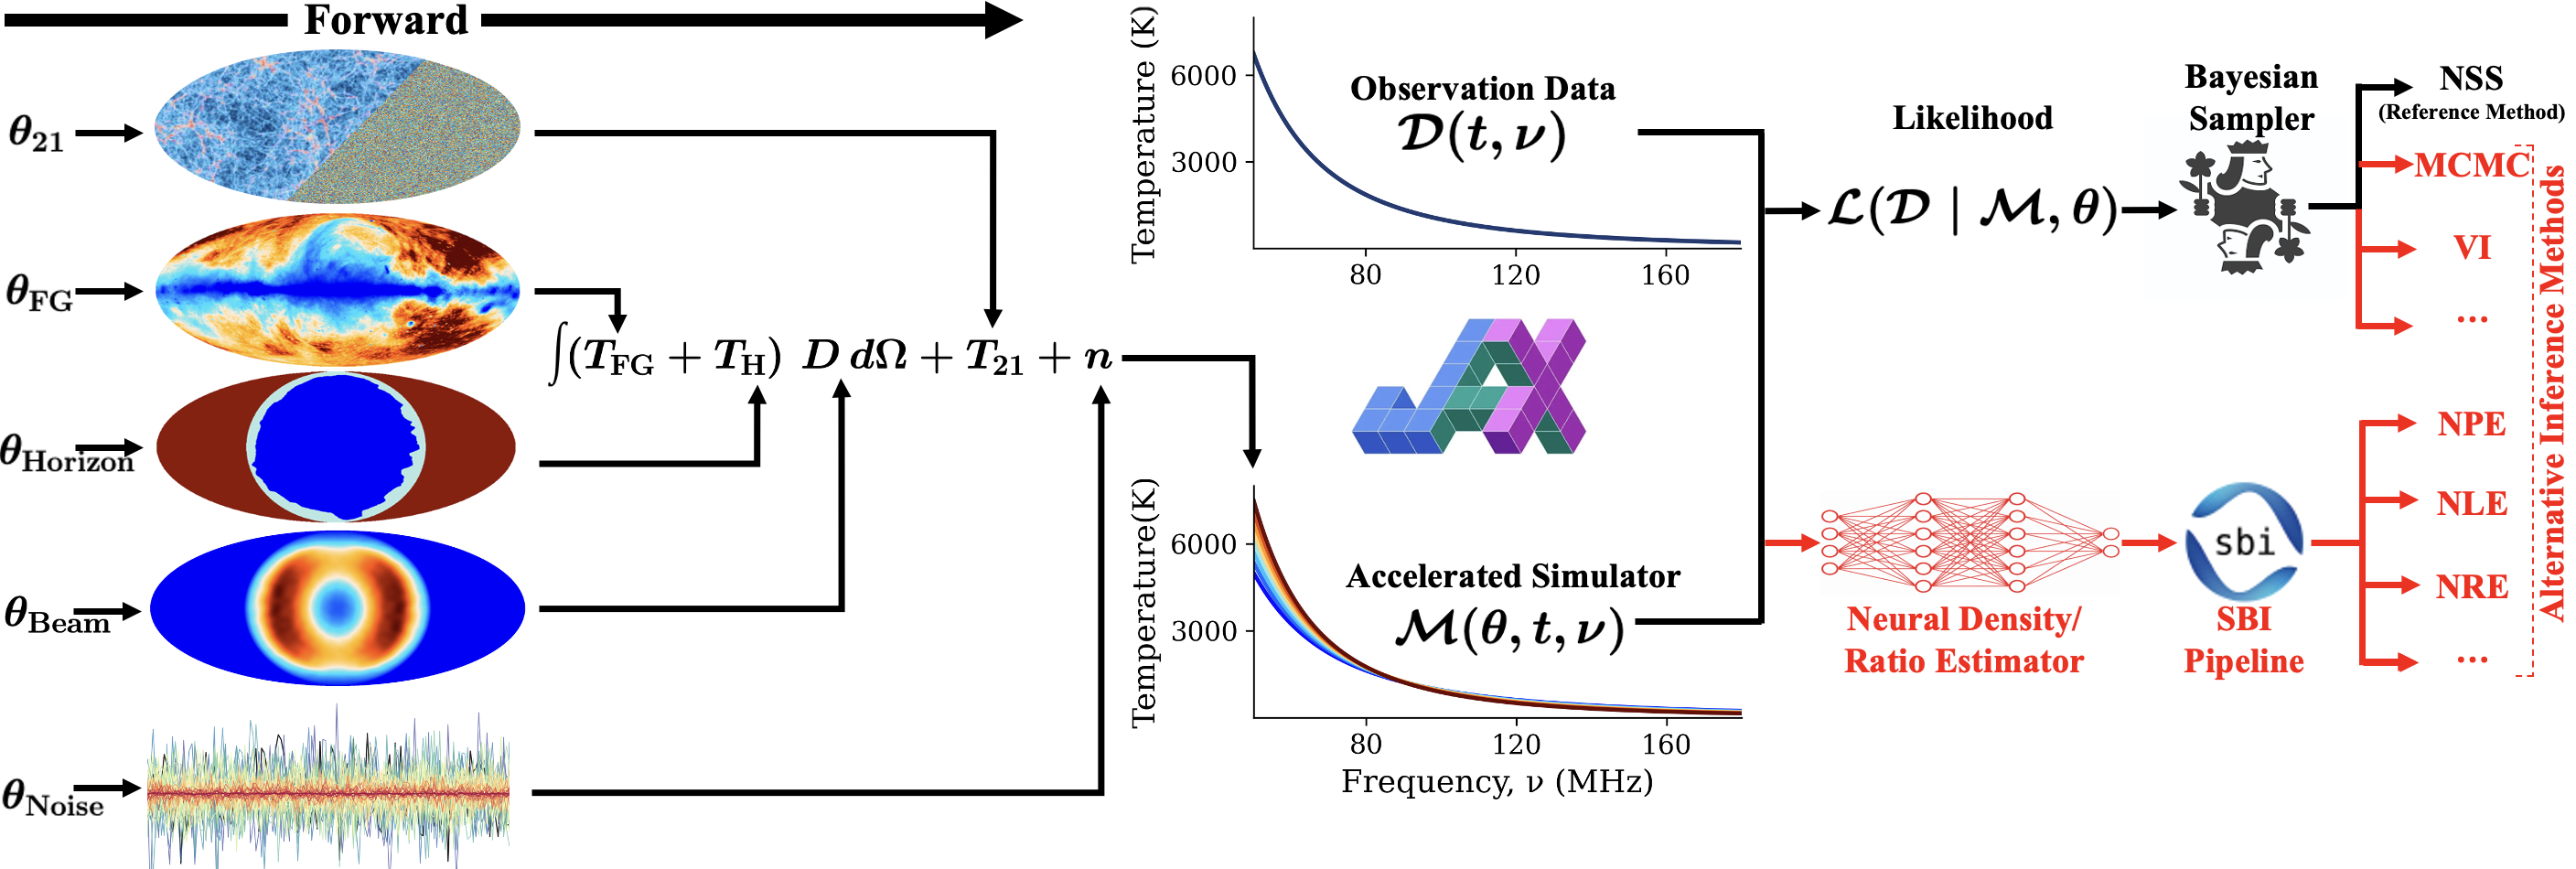
\includegraphics[width=0.9\linewidth,height=46mm]{figures/reach_inference_pipeline.png}
\caption{REACH's hybrid generative model (top) and accelerated inference framework (bottom), combining neural emulation, physically informed foreground modelling and a surrogate representation of antenna uncertainty. Figures 1 and 2 from Tutt et al. (2026c).}
\label{fig:reach}
\end{figure}
 By reformulating the mathematical evaluation and integrating a nested-sampling implementation optimised for parallel GPU execution, my work has enabled numerous extensions to the modelling and Bayesian validation framework across the collaboration (Tutt et al., 2026a). One such extension was the integration of physically informed surrogate models for the complex electromagnetic response of the antenna. The central challenge was to construct a model expressive enough to capture physically plausible instrumental variation, yet sufficiently constrained by physics to preserve the identifiability of the cosmological signal. To address this, I developed a novel method for learning a latent representation of the beam variations from computational electromagnetic simulations, compressing the beam parameterisation by two orders of magnitude and allowing the associated uncertainty to be analytically marginalised during inference (Tutt et al., 2026b).


Overall, the framework unifies astrophysics and computational electromagnetics through neural emulation, physics-informed parameterisations and latent-space representations, reducing model evaluation from approximately 2.8 hours of wall time (1,608 CPU-core hours) to 0.14 milliseconds on a single GPU, a speed-up of \(7.2\times10^7\). In addition, it provides a timely benchmark for sampling algorithms, simulation-based inference and variational inference, enabling their efficiency and reliability to be assessed on the complex posterior geometries encountered in realistic scientific applications (Tutt et al., 2026c).




Upcoming interferometric 21-cm experiments such as the Square Kilometre Array bring a further challenge of scale, with exascale data-processing demands and models requiring millions of parameters. To meet this challenge, I have led the mathematical reformulation and computational scaling of \href{https://jacobtutt.github.io/BayesEoR-JAX/dev/}{\color{awesome}BayesEoR}, a Bayesian framework for joint signal and foreground inference from interferometric visibilities. The central advance is to enable the use of covariance derived from a physical generative model, capturing high-dimensional correlations omitted by the phenomenological Gaussian process kernels commonly used. Drawing on methods for optimal statistical compression, I introduced a noise-informed Karhunen–Loève expansion into the framework, collapsing the parameterisation of this prior-predictive uncertainty into a statistically optimal latent space and making analytical marginalisation computationally tractable while controlling the discarded uncertainty relative to observational noise. Constructed once and reused throughout inference, this representation amortises its construction cost across subsequent likelihood evaluations. For a realistic observational configuration, this reduces the joint parameter space from over 300,000 to under 10,000 and cuts the computational cost by three orders of magnitude, enabling posterior inference and Bayesian evidence evaluation in approximately 20 GPU-minutes (Tutt et al., in prep.).

\noindent\begin{minipage}{\linewidth}
\centering
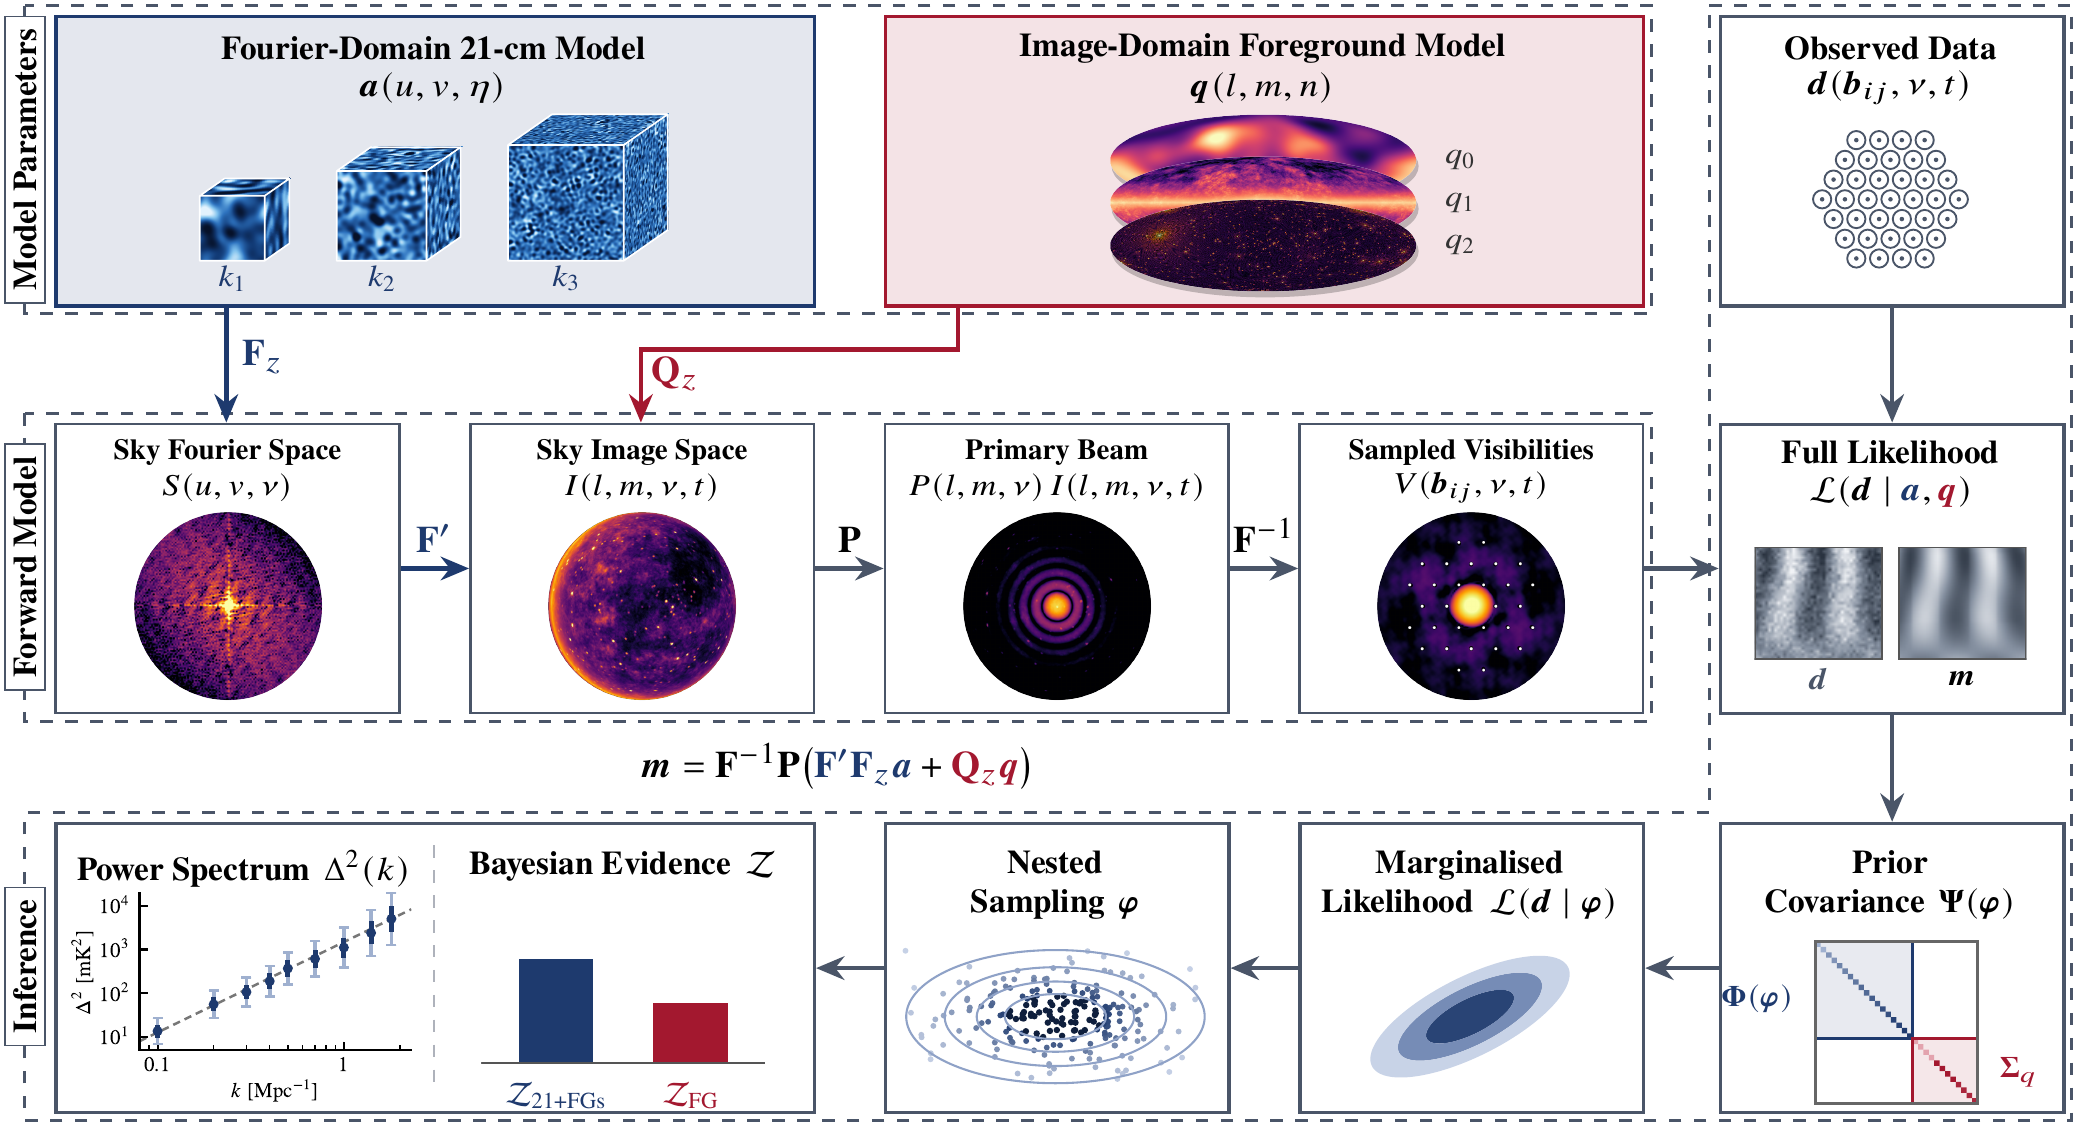
\includegraphics[width=0.9\linewidth,height=74.5mm]{figures/bayeseor_pipeline.png}\par\vspace{1mm}
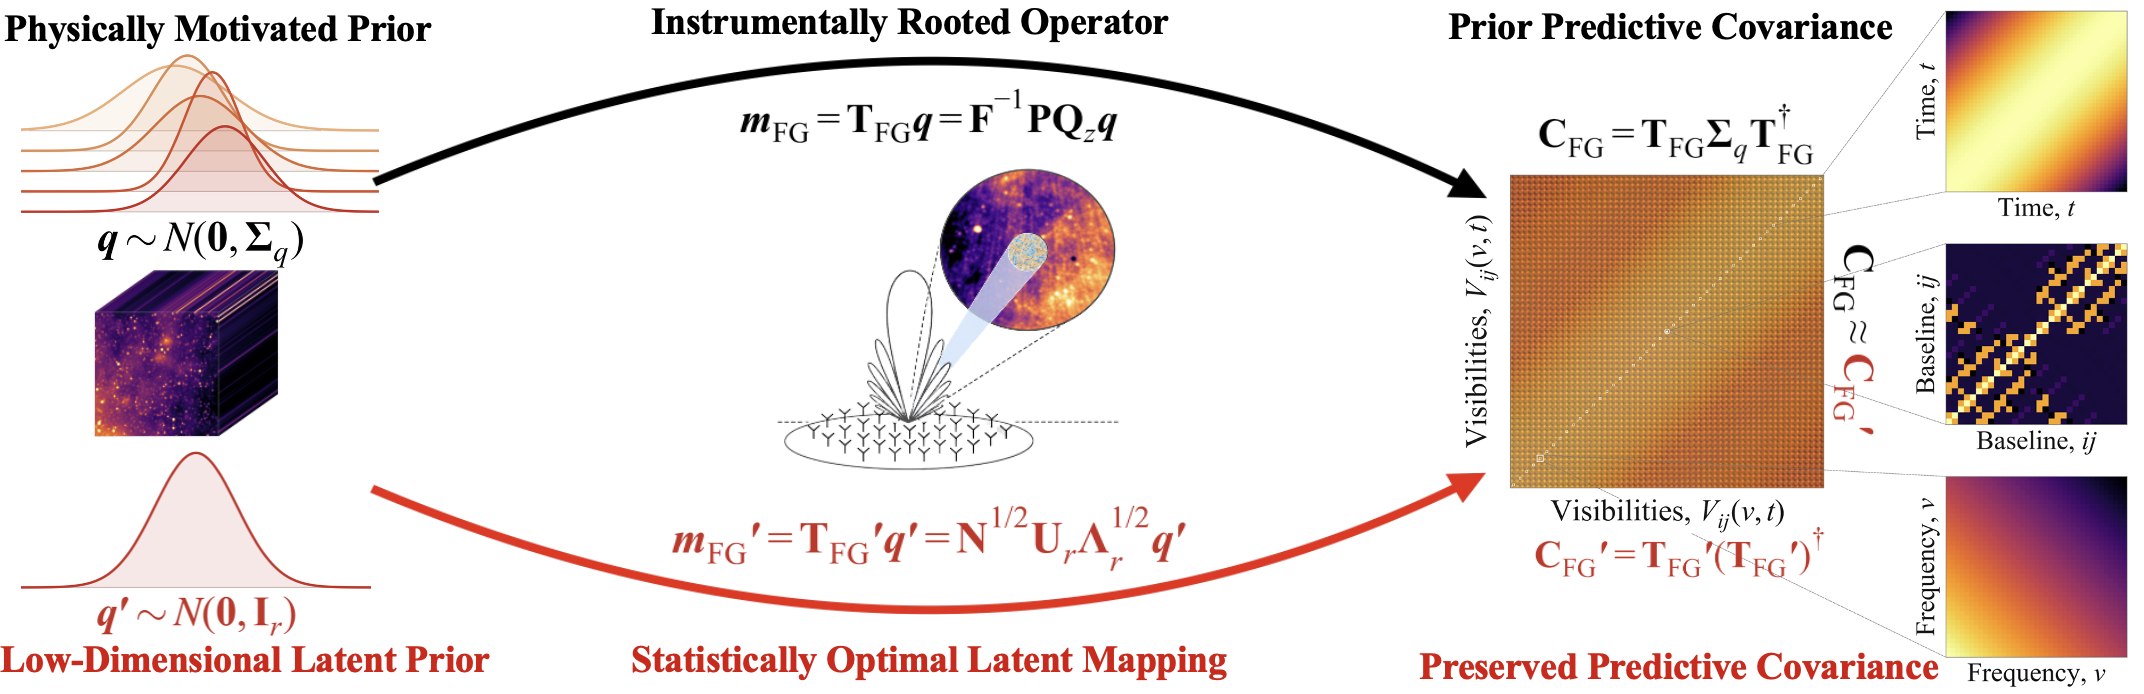
\includegraphics[width=0.9\linewidth,height=39.5mm]{figures/bayeseor_latent_compression.png}
\captionof{figure}{BayesEoR's joint forward model and inference workflow (top), and the compression of physically derived foreground uncertainty into a low-dimensional latent representation (bottom). Figures 2 and 3 from Tutt et al. (in preparation).}
\label{fig:bayeseor}
\end{minipage}

\newpage

Overcoming the bottleneck in BayesEoR led me to develop JAXMg, in collaboration with the Flatiron Institute's Center for Computational Quantum Physics. Our work in cosmology and quantum many-body physics had converged on the same computational challenge: solving large dense systems beyond the memory capacity of a single compute node. JAXMg addresses this by bringing distributed matrix factorisations and linear solves directly into JAX, allowing these computations to scale across multiple GPUs and nodes (Tutt \& Wiersema, 2026). With \href{https://pepy.tech/projects/jaxmg}{22,000 downloads} and \href{https://github.com/flatironinstitute/jaxmg}{114 GitHub stars}, JAXMg now supports research across computational physics, including quantum variational Monte Carlo (Wiersema, 2026; Wan, Wiersema \& Zhang, 2026), where its solvers underpin distributed optimisation in \href{https://github.com/netket/netket/tree/main}{NetKet} and \href{https://github.com/tachys-dev/tachys/tree/main}{tachys}, two leading libraries in the field. Ongoing development targets wider integration, including elliptic PDE solvers (Melia et al., 2025), computational electromagnetics (Gueuning et al., 2026) and Gaussian process inference (Pinder \& Dodd, 2022).

\noindent\begin{minipage}{\linewidth}
\centering
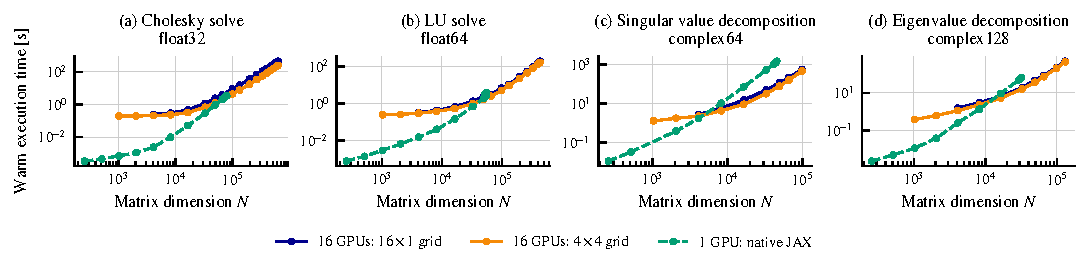
\includegraphics[width=\linewidth]{figures/jaxmg_benchmark_row.pdf}
\captionof{figure}{JAXMg benchmarks on 16 NVIDIA H100 GPUs across four nodes, comparing two process-grid layouts with native JAX on one GPU.}
\label{fig:jaxmg}
\end{minipage}

My current work explores simulation-based inference across global and interferometric 21-cm cosmology, where increasing model dimensionality motivates moving beyond conventional posterior sampling. Drawing inspiration from field-level inference, I am investigating how to scale marginal neural posterior estimation to problems involving hundreds of thousands of nuisance parameters, removing the need for repeated dense linear solves while allowing additional sources of uncertainty to be incorporated. Alongside this, I am exploring latent diffusion models and flow matching for the generation and super-resolution of three-dimensional cosmological fields, combining compressed representations with the flexibility to capture complex, non-Gaussian structure. These directions reflect the theme that runs through all of my research: scaling statistical and numerical methods without sacrificing rigorous uncertainty quantification. Whether through physically derived representations, distributed computation or amortised inference, my aim is to make principled inference tractable at scales previously out of reach, and to ensure that its conclusions can be trusted.

\begin{samepage}
\lettersection{References}
\color{black}
\begingroup
\fontsize{9pt}{11pt}\selectfont
\begin{itemize}[topsep=0pt,itemsep=2pt,parsep=0pt]
\item Tutt et al. (2026a). Optimizing foreground modelling for global 21-cm cosmology with GPU-accelerated nested sampling. MNRAS, 550, stag1101. \enskip\textbullet\enskip \href{https://arxiv.org/abs/2603.13196}{\color{awesome}arXiv:2603.13196}
\item Tutt et al. (2026b). Towards end-to-end Bayesian forward models in global 21-cm cosmology: surrogate modelling and marginalisation of beam uncertainty. \href{https://arxiv.org/abs/2608.18962}{\color{awesome}arXiv:2608.18962}.
\item Tutt et al. (2026c). A Cross-Domain Simulator and Benchmark for Uncertainty Quantification in Global 21-cm Inference. Sim2Science: ML with Imperfect Scientific Models, NeurIPS 2026. \enskip\textbullet\enskip \href{https://jacobtutt.github.io/assets/pdf/tutt_2026_sim2sci.pdf}{\color{awesome}PDF}
\item Tutt et al. (in preparation). An Optimal Latent Space for Amortised Bayesian Uncertainty Quantification and Evidence Evaluation in Interferometric Visibilities. \enskip\textbullet\enskip \href{https://jacobtutt.github.io/assets/pdf/tutt_2026_bayeseor.pdf}{\color{awesome}Draft PDF}
\item Tutt, J. \& Wiersema, R. (2026). JAXMg: A multi-GPU linear solver in JAX. \enskip\textbullet\enskip \href{https://arxiv.org/abs/2601.14466}{\color{awesome}arXiv:2601.14466}
\item Wiersema, R. (2026). Numerical simulation of D-Wave's quantum advantage experiment with time-dependent variational Monte Carlo. \enskip\textbullet\enskip \href{https://arxiv.org/abs/2609.01719}{\color{awesome}arXiv:2609.01719}
\item Wan, Z.-Q., Wiersema, R. \& Zhang, S. (2026). Removing nodal and support-mismatch pathologies in Variational Monte Carlo via blurred sampling. Physical Review X, 16, 031059. \enskip\textbullet\enskip \href{https://doi.org/10.1103/jrn5-gv19}{\color{awesome}DOI}
\item Melia et al. (2025). jaxhps: An elliptic PDE solver built with machine learning in mind. Journal of Open Source Software, 10(115), 8549. \enskip\textbullet\enskip \href{https://doi.org/10.21105/joss.08549}{\color{awesome}DOI}
\item Gueuning et al. (2026). A Fast Direct Solver for Mutual Coupling Analysis of Large Arrays of Reflector Antennas. \enskip\textbullet\enskip \href{https://arxiv.org/abs/2604.10239}{\color{awesome}arXiv:2604.10239}
\item Pinder, T. \& Dodd, D. (2022). GPJax: A Gaussian Process Framework in JAX. Journal of Open Source Software, 7(75), 4455. \enskip\textbullet\enskip \href{https://doi.org/10.21105/joss.04455}{\color{awesome}DOI}
\end{itemize}
\endgroup
\end{samepage}

\end{cvletter}
\end{document}
